%% Manuscript prepared with the IEEEtran class (journal mode) for submission to
%% IEEE Transactions on Learning Technologies. Compile with: latexmk -pdf main.tex
\documentclass[journal]{IEEEtran}

\usepackage[T1]{fontenc}
\usepackage[utf8]{inputenc}
\usepackage{amsmath,amssymb}
\usepackage{graphicx}
\usepackage{booktabs}
\usepackage{multirow}
\usepackage{array}
\usepackage{textcomp}
\usepackage{url}
\usepackage[hidelinks]{hyperref}
\hypersetup{pdftitle={Effect of a Multi-Agent LLM-Based Methodological Mentoring System on the Quality of Engineering Thesis Projects},pdfauthor={Aguilar Idrogo, Aguilar Alayo, Cueva Chavez}}

\newcolumntype{L}[1]{>{\raggedright\arraybackslash}p{#1}}
\newcolumntype{C}[1]{>{\centering\arraybackslash}p{#1}}

\begin{document}

\title{Effect of a Multi-Agent LLM-Based Methodological Mentoring System on the Quality of Engineering Thesis Projects: A Longitudinal Quasi-Experiment}

\author{Clever~Josu\'e~Aguilar~Idrogo,
        Alessia~Vidamilagros~Aguilar~Alayo,
        and~Walter~Manuel~Cueva~Ch\'avez%
\thanks{Manuscript received November 5, 2026. This work received no external funding. \textit{(Corresponding author: Clever Josu\'e Aguilar Idrogo.)}}%
\thanks{The authors are with the Computer and Systems Engineering Program, Faculty of Engineering, Universidad Privada Antenor Orrego, Trujillo 13008, Peru (e-mail: cleverjosue1@gmail.com).}}

\markboth{IEEE Transactions on Learning Technologies}%
{Aguilar Idrogo \MakeLowercase{\textit{et al.}}: Multi-Agent Methodological Mentoring and the Quality of Engineering Thesis Projects}

\maketitle

\begin{abstract}
Undergraduate engineering thesis projects are frequently returned with methodological observations. This study determined the effect of MentorIA, a multi-agent methodological mentoring system based on large language models, on the methodological quality of thesis projects in a Research Project course at a Peruvian engineering faculty during the 2026-2 semester. A mixed-methods, longitudinal quasi-experimental design with a nonequivalent control group was applied to two intact sections taught by the same instructor (16 control and 20 experimental thesis projects). Traditional mentoring was diagnosed through interviews with six advisors. Quality was measured in weeks 4 to 9 with a 100-item dichotomous rubric in 15 dimensions, validated by seven experts (Aiken's $V$ between .81 and 1.00) and applied by a blind panel of three language-model judges with majority voting; argumentative quality was assessed with Toulmin's model. At baseline the groups did not differ in the quality of the common core of dimensions (71.2\% vs. 78.5\%, $p = .057$) but did in traceability, favoring the control group. Quality increased in 32 of 36 projects (median $+13.0$ points, $p < .001$). The weekly slope of the experimental group was 3.10 points higher ($p < .001$), and the effect on the change in quality was large (Cohen's $d = 1.32$, 95\% CI $[0.60, 2.05]$), concentrated in the problem description and in the dimensions written during the intervention. Cumulative use (215 queries) was unrelated to improvement ($\rho = -.14$). Availability of the system as a complement to advising was associated with a more favorable evolution of methodological quality, without evidence of a dose--response relationship.
\end{abstract}

\begin{IEEEkeywords}
Argument mining, higher education, large language models, methodological quality, multi-agent systems, quasi-experiment, thesis supervision.
\end{IEEEkeywords}

\IEEEpeerreviewmaketitle

\section{Introduction}

\IEEEPARstart{I}{n} the Faculty of Engineering of Universidad Privada Antenor Orrego (UPAO), the Research Project course is the stage in which students of the Computer and Systems Engineering program formulate the thesis project with which they will apply for their professional degree, under a model of individualized advising. That model has a structural limitation: advising is organized in scheduled sessions within a fixed timetable and offers no channel of methodological guidance at the moment a doubt arises, so unresolved gaps accumulate and propagate through the document. A condition typical of engineering education adds to this: students tend to conceive the project from the technological solution they want to build rather than from the scientific problem they intend to solve, which inverts the methodological order and produces recurrent errors in the problem formulation, the definition of variables, and the research design. According to the advisors of the faculty, more than half of the projects submitted for the first time are returned with substantive methodological observations. The problem is not confined to one institution: in a Peruvian public university, 80\% of the approved undergraduate theses showed a merely acceptable methodological quality, with deficiencies attributed in part to the guidance received \cite{estrada2022}, and studies on the difficulties of Peruvian thesis writers have been built from the finished document or from the student's voice, without the perspective of the advisor \cite{perdomo2022,vilca2023}. Undergraduate thesis supervision, moreover, has received far less research attention than doctoral supervision \cite{agricola2021}.

Pedagogical conversational agents have been proposed as a mechanism for continuous, personalized, and scalable support in higher education, with applications that include mentoring \cite{yusuf2025}. The evidence on their effect on research writing, however, is heterogeneous and depends on the architecture of the tool. A conversational agent without a specialized architecture tended to operate as a dispenser of resources and did not sustain cognitively deep interactions when tutoring research projects \cite{ortega2021}; a basic chatbot had limited adoption and frequent failures with complex content questions in an academic research course in Lima \cite{arredondo2020}; and the spontaneous use of ChatGPT produced no significant differences in the quality of academic texts against a nonequivalent control group \cite{apolin2024}. In contrast, a structured four-session intervention with ChatGPT raised from 2.8\% to 80.6\% the proportion of graduate students with an adequate level in the formulation of research projects, although with a pre-experimental design without a comparison group \cite{hinojosa2024}. A systematic review with meta-analysis recommends evaluating these effects over time to distinguish them from a novelty effect \cite{deng2025}.

Multi-agent systems based on large language models (LLMs) offer an alternative to single-model conversational assistance. Debate among several agents that propose and critique answers improved the factual accuracy and reasoning of language models \cite{duy2024}; in a quasi-experiment with computer science students, the condition with multi-agent debate obtained a relative learning gain of 29.78\%, with a medium effect size \cite{duj2025}; the separation of roles between critical agents and a judge reduced the pedagogical sycophancy of automated tutors \cite{sadhu2025}; and decomposing essay evaluation into specialized agents guided by a rubric raised agreement with human raters \cite{jordan2025}. Panels of LLM judges, however, exhibit a self-preference bias when evaluator and generator belong to the same model family \cite{panickssery2024}. In addition, the argumentative structure of student texts can be identified automatically and reproducibly \cite{stab2017}, and feedback on that structure improved the quality of persuasive texts \cite{wambsganss2020}; those procedures, however, have been developed on essays rather than on the argumentative sections of a research project.

Five gaps follow from this review. First, the scarcity of diagnoses of methodological deficiencies from the perspective of the engineering advisor, organized by section of the project. Second, the measurement of methodological quality at a single moment or with only two measurements, which does not reveal when the trajectories of the groups separate. Third, the predominance of interventions with a single general-purpose conversational model, with little controlled evidence on specialized multi-agent systems. Fourth, the recording of actual tool use for descriptive purposes, without linking it to the quality of a research product. Fifth, the absence of a computational assessment of argumentation in research projects and of its relation to the methodological quality of the document.

The general objective of this study was to determine the effect of a multi-agent methodological mentoring system on the methodological quality of the thesis projects of engineering students at UPAO in the 2026-2 semester. The specific objectives were: (SO1) to explore the recurrent methodological deficiencies of traditional mentoring from the advisors' perspective; (SO2) to measure the evolution of the methodological quality of the projects across weekly measurements; (SO3) to determine the relation between the level of use of the system and the improvement in quality in the experimental group; (SO4) to compare the evolution of quality between the control and experimental groups; and (SO5) to compare between groups the evolution of the argumentative quality of the problem description and the justification, assessed computationally with Toulmin's model. The general hypothesis stated that the multi-agent system has a positive and statistically significant effect on the methodological quality of the projects; specific hypotheses H2 to H5 stated, respectively, that quality increases across measurements, that the level of use is positively related to improvement, that the experimental group shows a greater evolution than the control group, and that argumentative quality increases more in the experimental group. The contributions are a controlled longitudinal evaluation of a specialized multi-agent system in a real course, an expert-validated rubric administered by an LLM panel with consistency reported at every measurement, and a computational index of argumentation for the sections of a research project.

\section{Materials and Methods}

\subsection{Design}

A mixed-methods, applied, explanatory study was conducted with a longitudinal quasi-experimental design with a nonequivalent control group \cite{hernandez2018}. The groups were two intact sections of the course; each section was randomly assigned, as a block, to one of the two conditions. The independent variable, exposure to the multi-agent system, was manipulated by making the system available only to the experimental group; the dependent variable, the methodological quality of the thesis project, was measured weekly in both groups with the same instrument and the same evaluation system. The design scheme was CG: $O_1 \rightarrow O_2 \rightarrow \cdots \rightarrow O_n$; EG: $O_1 \rightarrow X \rightarrow O_2 \rightarrow X \rightarrow \cdots \rightarrow O_n$, where $O_1$ is the baseline measurement of week 4, $X$ is the use of the system between consecutive measurements, and $O_2$ to $O_n$ are the successive measurements. Since both groups start the course with an institutional template without assessable text, equivalence was verified at the baseline measurement, when both had already written the first dimensions of the project. Internal validity was addressed with three strategies: verification of baseline homogeneity on the common core of dimensions developed by both groups; comparison of the trajectories of both groups on the same dimensions; and a dose--response analysis within the experimental group, which holds section-specific factors constant.

\subsection{Population and Sample}

The unit of analysis was the thesis project, not the student, since the dependent variable is measured on the document and each project may be written by one or two students. The population consisted of the projects of the Research Project course of the Faculty of Engineering at UPAO in the 2026-2 semester, taught in three sections with 31, 30, and 33 enrolled students. The sample, nonprobabilistic and purposive, comprised the two sections taught by the same instructor, with the same syllabus and submission calendar, which avoids confounding the instructor effect with the intervention; each section formed 20 projects, and within each section all projects whose students authorized their participation were included. Projects that submitted an assessable version, with the students' own text in at least one dimension of the rubric, at the baseline measurement were included in the analysis. Four control-group projects still contained only the course template at that measurement and were excluded from the analytic sample, which comprised 36 projects: 16 in the control group and 20 in the experimental group. For the fifth specific objective, the unit of analysis was the complete argumentative section of each project (problem description and justification), defined as one containing at least 80 words written by the students with at least 60\% of them in complete sentences.

\subsection{Intervention: The MentorIA System}

In addition to traditional advising, the experimental group had access to MentorIA, a multi-agent methodological mentoring system deployed as a cloud web application to which each student logged in with an individual account. The system receives the student's project in PDF, Word, or plain-text format, indexes it in a session vector store, and evaluates it against a rubric structured by explicit methodological criteria; the student declares which parts are to be reviewed, so that what has not been submitted is not graded. Its core is a network of LLM-based agents with separate roles, orchestrated by a supervisor that decides at each turn which agent intervenes: an Auditor that scores the rubric criteria with structured output, a Methodologist that reviews rigor and cross-section coherence (problem, objectives, hypotheses, variables, and design), a Writer that proposes improved text supported by retrieval-augmented access to methodological literature, and a debate round between the Writer and the evaluators, with loop protection. The student's original document is never modified: improvements are presented as proposals that the student decides whether to incorporate. Four interaction types were available: quick queries, quick improvements of a fragment, section reviews, and full-project reviews. According to the technology readiness scale adapted by the Peruvian National Council for Science, Technology and Technological Innovation (CONCYTEC) \cite{concytec2022}, the system is at TRL~7, since it is deployed and in real use during the course. Its architecture, configuration, and knowledge base remained fixed throughout the study. The system was available in trial mode from week 2; the intervention is counted from the baseline measurement, from week 5 to week 9.

\subsection{Instruments and Measures}

\subsubsection{Methodological Quality Rubric}
Methodological quality was measured with a rubric of 100 dichotomous items (met = 1; not met = 0) grouped in 15 dimensions, built for the study from the criteria of Hern\'andez Sampieri and Mendoza Torres \cite{hernandez2018} and from the definition of methodological quality as the degree of compliance with the rigor standards that sustain validity \cite{chacon2023}. The dimensions are: title (D1); problem description and delimitation (D2); problem formulation (D3); objectives (D4); justification, importance, and feasibility (D5); limitations (D6); theoretical framework (D7); hypotheses (D8); variables and operationalization (D9); consistency matrix (D10); research type, approach, and scope (D11); research design (D12); population, sample, and sampling (D13); data collection techniques and instruments (D14); and data processing and analysis techniques (D15). An item is scored as met only when the element is explicitly stated in the text. Content validity was established through the judgment of seven experts holding a master's or doctoral degree and with 4 to 15 years of experience in research or thesis advising, in two rounds, following the template of Escobar-P\'erez and Cuervo-Mart\'inez \cite{escobar2008}, with Aiken's $V$ coefficient \cite{aiken1980} and an acceptance criterion of $V \geq .80$ per item for pertinence, relevance, and clarity, and per dimension for sufficiency. In the first round the coefficients ranged from .67 to 1.00 (mean .96) and twelve items did not reach the criterion; 27 items were reworded without changing the number of items or dimensions. In the second round all items reached the criterion, with values between .81 and 1.00 (mean .98) and 55 items with $V = 1.00$ on the three criteria; sufficiency per dimension ranged from .81 to 1.00. The main variable was the \emph{written quality}: the percentage of criteria met over the criteria of the dimensions the project has developed, which separates the quality of what is written from the extent of progress; when a project develops all 15 dimensions it coincides with the total score from 0 to 100. Two derived measures were also computed: the quality in the common core of dimensions developed by both groups, and the traceability among title, problem, and objectives, calculated as the percentage met of six correspondence items.

\subsubsection{Multi-Agent Evaluation System}
The rubric was administered at every measurement by an evaluation system built for the study, which made the weekly evaluation of the 40 projects feasible and avoided the conflict of interest of having the advisor grade the projects under his own supervision. The system consists of a panel of three LLM judges of different capacity (gpt-4o-mini, gpt-4.1-mini, and gpt-4.1), orchestrated in a network architecture with LangGraph. Each judge independently evaluates the items of the dimensions containing the students' own text, restricting its judgment to the explicit criteria of the instrument and to the textual evidence of the document; the score of each item is obtained by majority vote. The three judges run with temperature 0 and a fixed seed. Evaluation is blind: before sending the text, the system masks names, identity documents, e-mail addresses, ORCID identifiers, and telephone numbers, and no judge receives the file name or the group of the project. Items of dimensions without the students' own text, including those that retain only the institutional template, are recorded as not met without consulting the panel. When a submission contains the same text as the previous one, the project keeps its score. As evidence of consistency, the percentage of unanimous decisions, Fleiss' kappa \cite{fleiss1971}, and Gwet's AC1 coefficient \cite{gwet2008} are reported at every measurement. According to the CONCYTEC scale \cite{concytec2022}, the evaluation system is at TRL~6, as a functional prototype operated by the researchers.

\subsubsection{Argumentation Index and Global Coherence}
The evaluation system computes two coherence indicators in which the language model does not assign the score: it identifies elements of the text, the system verifies them automatically, and the score is obtained with a fixed rule. The argumentation index is based on the six components of Toulmin's model \cite{toulmin2003}: claim, data, warrant, backing, qualifier, and rebuttal, whose presence distinguishes an elaborated argument from a list of claims and data \cite{erduran2004,qin2010}. In its version 2.0, used for the fifth objective, the complete section is divided into paragraphs and numbered units, and the gpt-4.1 model (temperature 0, fixed seed) identifies the author's claims and, for each one, the units of any paragraph that act as its data, warrant, backing, or rebuttal; the system verifies that the identifiers exist and that each warrant connects a valid datum of the same claim. The \emph{structural index} (component types present out of six, as a percentage), the \emph{elaboration index} (mean, over the claims, of the proportion of the five supporting components each claim has), the argumentation level from 0 to 5 adapted from Erduran \emph{et al.} \cite{erduran2004}, and the component profile are computed. Its test--retest stability, verified on 58 sections of week 4, was 80.6\% for the functions assigned to 1\,215 units and 65.4\% for the links, with an intraclass correlation coefficient ICC(2,1) of .77 for both indices, interpreted according to Koo and Li \cite{koo2016}. The global coherence of the project is obtained from the contradictions between two parts of the document that the model lists with a literal quotation and that the system keeps only if both quotations exist in the text; a score from 1 to 5 is assigned by rule according to the number and severity of the contradictions.

\subsubsection{System Usage Logs}
The actual delivery of the intervention was verified with the automatic logs of the system, organized by project and academic week: number of queries by type (main dose indicator), days with queries, minutes in sessions with queries, and sessions without messages. A session is a block of activity without pauses longer than 30 min; minutes of sessions without messages are reported only as exposure and are included in a sensitivity analysis. A week without queries is recorded as zero dose. Accounts were assigned to projects from the authors on the cover page and verified with the documents uploaded.

\subsubsection{Semi-Structured Interview}
For the first objective, an interview guide, reviewed by expert judgment, was applied to six advisors and reviewers of thesis projects of the Faculty of Engineering, oriented to identifying methodological deficiencies, limitations of traditional mentoring, and the functionalities expected from a support tool. Transcripts were processed by identifying meaning units, coding, grouping into categories, and triangulation \cite{vives2021}; the rigor criterion was category saturation and convergence among informants.

\subsection{Procedure}

The course began in week 1 with the institutional project template without content. Each group presented its progress in its weekly class session, on Mondays for the experimental group and on Thursdays for the control group, so both were measured with the same number of sessions. Measurements were taken in weeks 4 (baseline), 5, 6, 7, and 9 of the semester; there was no measurement in week 8 because the projects presented no progress. At each measurement the evaluation system segmented the submission into the rubric dimensions with fixed rules, verified the segmentation against the original document, scored the dimensions with the students' own text, and computed the argumentation index and global coherence. System use in each week was related to the change in quality in the interval ending in that week. Statistical processing and figures were produced in Python with the pandas and Seaborn libraries.

\subsection{Data Analysis}

Qualitative information was processed by thematic analysis. For quantitative data, the mean, median, and standard deviation of written quality by group and measurement, and the percentage of achievement per dimension, were reported. Baseline homogeneity was verified with a decision rule fixed in advance: normality per group with the Shapiro--Wilk test \cite{shapiro1965} and homogeneity of variances with the median-centered Levene test \cite{brown1974}; depending on the result, Student's $t$, Welch's $t$, or the Mann--Whitney $U$ test, with a significance level of .05 and the effect size as Hedges' $g$ \cite{hedges1981} or Cliff's $\delta$ \cite{cliff1993}, interpreted according to Cohen \cite{cohen1988} and Romano \emph{et al.} \cite{romano2006}. H2 was tested with the one-sided Wilcoxon signed-rank test on the change in quality of each project between week 4 and week 9, computed on the dimensions written at both measurements. H3 was tested with the one-sided Spearman correlation between cumulative use (queries) and the total change in quality in the experimental group; as a complement, the correlations per interval and a mixed-effects model with the use of the week and of the previous week were reported. H4 was tested with a linear mixed-effects model with a random intercept per project, quality $\sim$ group $\times$ week, on the quality in the dimensions developed by at least half of the projects of each group at each measurement; $H_0$ is rejected if the interaction favors the experimental group with one-sided $p < .05$, and the test was complemented with the Mann--Whitney $U$ test on the total change. H5 was tested with the one-sided Mann--Whitney $U$ test on the change in the elaboration index of each section between the first and the last measurement with the section complete, with Holm's correction \cite{holm1979} for the two sections; it is partially accepted if $H_0$ is rejected in only one section. The general hypothesis was tested independently with Cohen's $d$ \cite{cohen1988} of the difference between groups in the change in quality in the common core between the baseline and final measurements, with its 95\% confidence interval and a one-sided test chosen with the same normality rule; $H_i$ is accepted if $d$ favors the experimental group, $d \geq 0.20$, and $p < .05$. Each hypothesis was decided with a single main test.

\subsection{Ethical Considerations}

Students of both sections authorized their participation in the study. Documents were anonymized before evaluation, and the interviewed advisors consented to the recording and analysis of the interviews. The mentoring system did not modify the students' documents, and its use was voluntary and complementary to the advising of the course.

\section{Results}

\subsection{Diagnosis of Traditional Mentoring}

Thematic analysis of the six interviews identified 151 meaning units, organized in 35 codes (29 a priori and 6 emergent) and grouped in 8 categories. Six categories reached full saturation across the six advisors: the general perception of the methodological level, the internal coherence and traceability of the project, the students' repetitive doubts, the divergence of criteria between advisors and examining boards, the minimum rigor criteria, and the frequency of project returns at the first submission, whose estimates ranged from 10\% to 70\% depending on the informant. Deficiencies concentrated in the methodological framework and the problem formulation, with high incidence, and in variables and indicators, with medium-high incidence; citation and format errors were rated as minor (Table~\ref{tab:interviews}). Advisors devote 5 to 8 h per month to repetitive doubts and 3 to 4 additional hours to out-of-hours queries, and described the punctual nature of advising as the main structural limitation. The functionalities they expect from a support tool are coherence review among problem, objectives, variables, and hypotheses, methodological guidance, evidence-based suggestions, and permanent availability, under two conditions of trust: traceability to verifiable sources and a strictly supporting role. An emergent code located part of the deficiencies in the rigidity of the institutional research model itself.

\begin{table}[!t]
\caption{Methodological Deficiencies by Project Section According to the Advisors}
\label{tab:interviews}
\centering
\footnotesize
\begin{tabular}{L{1.9cm}L{4.4cm}L{1.2cm}}
\toprule
Project section & Main finding & Incidence \\
\midrule
Problem formulation & Poorly delimited and superficial problem; does not reflect the full problematic situation & High \\
Methodological framework & Predominance of pretest--posttest schemes; unawareness of alternatives; rigid sequences & High \\
Variables and indicators & Poorly defined or non-operationalized variables; unclear indicators & Medium-high \\
Objectives & Poorly sized specific objectives, not aligned with the general objective & Medium \\
Hypotheses & Vague or conjectural hypotheses; not aligned with the problem & Medium \\
Title & Ambiguity, redundancy, and lack of traceability with objectives and hypotheses & Medium \\
Theoretical framework & Incomplete references; lack of critical analysis of prior work & Medium \\
References and citation & Minor APA errors, correctable with tools & Low \\
\bottomrule
\end{tabular}
\\[2pt]
\raggedright\scriptsize Synthesis of the thematic analysis of six semi-structured interviews with advisors of the Faculty of Engineering at UPAO; 151 meaning units, 35 codes, and 8 categories.
\end{table}

\subsection{Baseline Equivalence of the Groups}

At the baseline measurement, all 20 experimental projects and 16 of the 20 control projects contained assessable text. The control group had written more dimensions on average (7.4 vs. 6.0) and had a higher total score (median 33.5 vs. 22.0 points), whereas the quality of everything written was similar (64.8\% and 66.8\%), which shows that the total score reflects progress rather than quality. Homogeneity was therefore verified on the common core of dimensions D1 to D5, developed by both groups. Quality in the common core was normal in both groups with homogeneous variances; traceability, the argumentation index, and global coherence were not normal (Shapiro--Wilk, $p < .001$). The groups did not differ significantly in the quality of the common core, in the argumentation index of the problem description, or in global coherence, but did differ in traceability, favoring the control group (Table~\ref{tab:baseline}); baseline homogeneity was therefore partial. The problem description was the core dimension with the lowest achievement in both groups (62\% in the control group and 55\% in the experimental group); the criteria most frequently unmet were the quantification of the current situation with an indicator, value, and source (11 of 16 and 11 of 18 projects), the support of the consequences of the problem (11 of 16 and 11 of 18), the statement of feasibility (8 of 14 and 10 of 11), and the formulation of specific problems as questions, unmet by all 18 experimental projects that had written the formulation and by 5 of the 14 control projects.

\begin{table*}[!t]
\caption{Comparison of Methodological Quality Between Groups at Baseline (Week 4)}
\label{tab:baseline}
\centering
\footnotesize
\begin{tabular}{L{4.2cm}L{3.1cm}L{3.1cm}L{2.2cm}cL{1.6cm}}
\toprule
Variable & Experimental group ($n = 20$) & Control group ($n = 16$) & Test & $p$ & Effect size \\
\midrule
Quality in the common core (\%) & $M = 71.2$ ($SD = 11.6$) & $M = 78.5$ ($SD = 10.2$) & $t(34) = -1.97$ & .057 & $g = -0.65$ \\
Traceability of the core (\%) & $Mdn = 83.3$ ($M = 75.9$) & $Mdn = 91.7$ ($M = 84.4$) & $U = 76.0$ & .012 & $\delta = -0.47$ \\
Argumentation index, problem description (\%) & $Mdn = 33.3$ ($M = 42.1$) & $Mdn = 33.3$ ($M = 42.7$) & $U = 140.0$ & .886 & $\delta = 0.03$ \\
Global coherence (1--5) & $Mdn = 5$ ($M = 4.90$) & $Mdn = 5$ ($M = 4.88$) & $U = 162.0$ & .904 & $\delta = 0.01$ \\
\bottomrule
\end{tabular}
\\[2pt]
\parbox{0.92\textwidth}{\raggedright\scriptsize $g$ = Hedges' $g$; $\delta$ = Cliff's delta (experimental vs. control group). For traceability the experimental group had 18 projects and for the argumentation index 17; for the argumentation index the control group had 16 complete sections. An index of 33.3\% equals two of the six Toulmin components. Levene's test was nonsignificant for all four variables.}
\end{table*}

Panel consistency was recorded at every measurement on the items submitted to the three judges (between 369 and 1\,512 items per group and measurement). Between 67.3\% and 76.7\% of the items received a unanimous decision; Fleiss' kappa ranged from .46 to .66, a moderate to substantial agreement according to Landis and Koch \cite{landis1977}, and Gwet's AC1 from .62 to .78.

\subsection{Evolution of Methodological Quality}

Quality on the dimensions each project had written in week 4 increased in both groups. Its median went, in the control group, from 64.6\% in week 4 to 77.8\%, 78.8\%, 77.7\%, and 79.4\% in weeks 5, 6, 7, and 9, and in the experimental group from 71.0\% to 73.8\%, 75.2\%, 81.5\%, and 82.4\%. In week 9, the median quality of everything written was 75.2\% in the control group and 81.9\% in the experimental group. In terms of progress, the experimental group went from a median of 5 to 12 written dimensions and from 22.0 to 63.0 points, and the control group from 8 to 11 dimensions and from 33.5 to 55.5 points. Between week 4 and week 9, quality on the dimensions written at both measurements increased in 32 of the 36 projects, decreased in 1, and did not change in 3, with a median change of $+13.0$ points (Table~\ref{tab:wilcoxon}); the increase was significant in both groups, so $H_0$ of H2 was rejected.

\begin{table}[!t]
\caption{Change in Methodological Quality Between Week 4 and Week 9 on the Dimensions Written at Both Measurements}
\label{tab:wilcoxon}
\centering
\scriptsize
\setlength{\tabcolsep}{3.5pt}
\begin{tabular}{lcccccccc}
\toprule
Projects & $n$ & $+/-/=$ & $Mdn$ W4 & $Mdn$ W9 & Change & $W$ & $p$ & $r$ \\
\midrule
All & 36 & 32/1/3 & 67.7 & 80.0 & $+13.0$ & 555.5 & $<.001$ & .86 \\
CG & 16 & 15/0/1 & 64.6 & 79.4 & $+11.3$ & 120.0 & $<.001$ & .88 \\
EG & 20 & 17/1/2 & 71.0 & 82.4 & $+14.3$ & 167.5 & $<.001$ & .84 \\
\bottomrule
\end{tabular}
\\[2pt]
\raggedright\scriptsize One-sided Wilcoxon signed-rank test ($H_1$: quality increases). CG = control group; EG = experimental group; $+/-/=$ = projects that improved, worsened, or did not change; $Mdn$ = median quality in percent; Change = median change in percentage points; $r = z/\sqrt{n}$.
\end{table}

By dimension, among the projects that wrote them, achievement in the problem description went from 55\% to 82\% in the experimental group and from 62\% to 59\% in the control group, and in the problem formulation from 67\% to 83\% and from 90\% to 84\%, respectively. In week 9, achievement in the theoretical framework was 92\% in the experimental group and 82\% in the control group; in hypotheses, 86\% and 74\%; in variables, 92\% and 76\%; research type and design showed the lowest achievement among the written dimensions (65\% and 51\% in the experimental group; 44\% and 32\% in the control group), and the three methodological dimensions were written by 6 to 8 experimental projects and 2 control projects (Fig.~\ref{fig:heatmap}).

\begin{figure*}[!t]
\centering
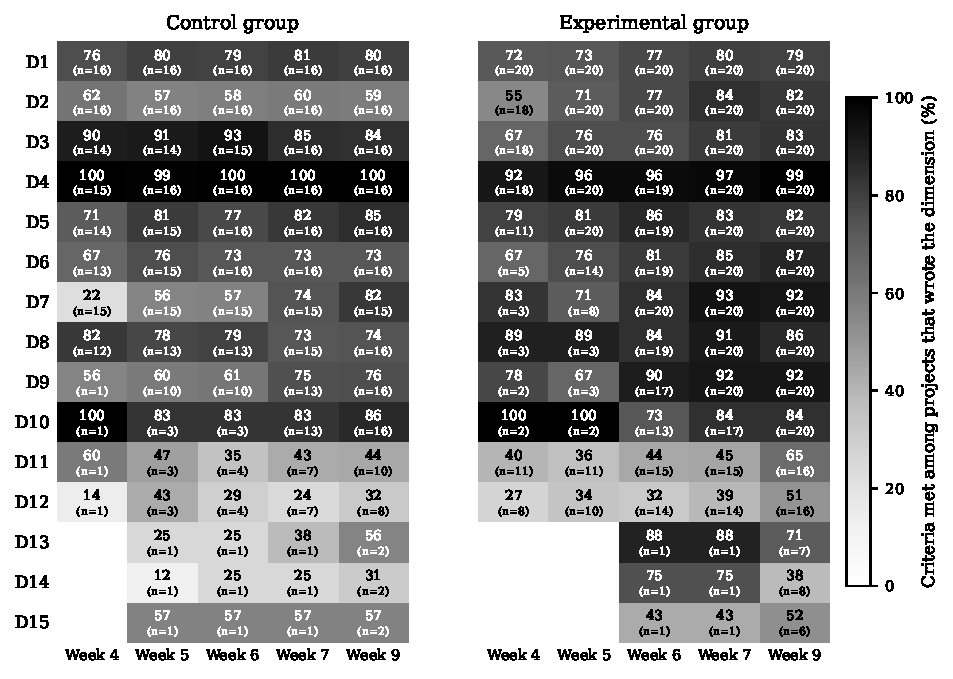
\includegraphics[width=0.92\textwidth]{figures/fig2_dimension_heatmap.pdf}
\caption{Achievement by rubric dimension from week 4 to week 9, by group. Percentage of criteria met among the projects that wrote each dimension at each measurement; in parentheses, the number of projects. D1 = title; D2 = problem description; D3 = problem formulation; D4 = objectives; D5 = justification; D6 = limitations; D7 = theoretical framework; D8 = hypotheses; D9 = variables; D10 = consistency matrix; D11 = research type; D12 = design; D13 = population and sample; D14 = techniques and instruments; D15 = data processing and analysis. Week 8 was not measured.}
\label{fig:heatmap}
\end{figure*}

\subsection{System Use and Its Relation to Improvement}

All 31 students of the experimental group had an account, and 18 of the 20 projects queried the system at least once between week 5 and week 9, with 215 queries in total: 98 in week 5 (17 projects), 22 in week 6 (8 projects), 72 in week 7 (9 projects), and 23 in weeks 8 and 9 (2 projects). Quick queries (106) and quick improvements (66) predominated, followed by full-project reviews (28) and section reviews (15). There were 76 sessions with queries (2\,272 min) and 104 sessions without messages (697 min). Use concentrated in a few projects: four of them accounted for 135 of the 215 queries. In none of the four intervals was the number of queries significantly related to the change in quality on the dimensions of the previous week (Spearman's $\rho$ between $-.20$ and .24; one-sided $p$ between .155 and .807), and the mixed-effects model of the change per interval (80 intervals) showed no effect of the use in the interval ($b = -0.07$ points per query, $p = .759$) or in the previous one ($b = -0.10$, $p = .709$). The correlation between cumulative use and the total change in quality between week 4 and week 9 was negative and nonsignificant ($\rho = -.14$, $p = .725$, $n = 20$), as it was for days with queries ($\rho = -.22$) and minutes in sessions with queries ($\rho = -.25$). The four projects with the highest use changed by $+3.2$, $+32.6$, $+8.7$, and 0.0 points, while three projects with fewer than five queries improved by more than 20 points (Fig.~\ref{fig:use}). Consequently, $H_0$ of H3 was not rejected.

\begin{figure}[!t]
\centering
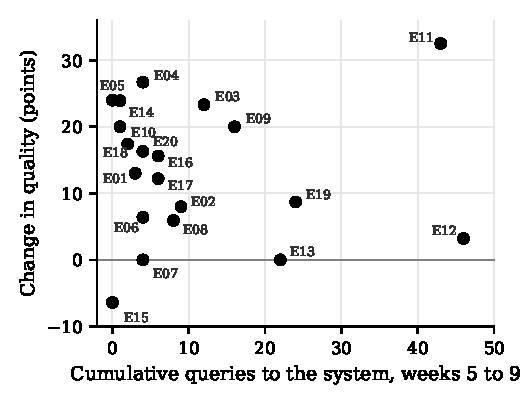
\includegraphics[width=\columnwidth]{figures/fig3_use_vs_change.pdf}
\caption{Cumulative use of the system versus change in quality between week 4 and week 9 in the experimental group ($n = 20$). The change is computed on the dimensions each project had written at both measurements. Spearman's $\rho = -.14$, one-sided $p = .725$.}
\label{fig:use}
\end{figure}

\subsection{Comparison of Trajectories Between Groups}

Quality in the dimensions developed by both groups was 78.5\% in the control group and 71.2\% in the experimental group in week 4 (D1--D5); 79.7\% and 79.5\% in week 5 (D1--D6); 72.4\% and 83.6\% in week 6 (D1--D9); 77.2\% and 88.2\% in week 7 (D1--D10); and 75.6\% and 83.9\% in week 9 (D1--D12). From week 6 onward the quality of the experimental group exceeded that of the control group at every measurement (Fig.~\ref{fig:core}). In the mixed-effects model, the quality of the experimental group started 2.22 points below that of the control group and its weekly slope was 3.10 points higher (Table~\ref{tab:mixed}), so $H_0$ of H4 was rejected. The total change on the dimensions each project had already written did not differ between groups (medians of $+14.3$ and $+11.3$ points; $U = 161.0$, $p = .494$, $\delta = 0.01$): both groups improved what they had already written to a similar extent, and the difference originated in the quality with which the experimental group wrote the dimensions incorporated after the baseline measurement.

\begin{table}[!t]
\caption{Linear Mixed-Effects Model of Quality in the Common Core, Week 4 to Week 9}
\label{tab:mixed}
\centering
\footnotesize
\begin{tabular}{L{3.0cm}rrcc}
\toprule
Term & $b$ & $SE$ & 95\% CI & $p$ \\
\midrule
Intercept (control group, week 4) & 78.09 & 1.86 & $[74.44, 81.74]$ & $<.001$ \\
Experimental group & $-2.22$ & 2.50 & $[-7.12, 2.67]$ & .373 \\
Week & $-0.64$ & 0.48 & $[-1.58, 0.31]$ & .187 \\
Experimental group $\times$ week & 3.10 & 0.65 & $[1.83, 4.37]$ & $<.001$ \\
\bottomrule
\end{tabular}
\\[2pt]
\raggedright\scriptsize 180 observations from 36 projects; random intercept per project (variance 26.42; residual variance 55.09). $b$ in percentage points; weeks are counted from the baseline measurement, so week 9 corresponds to the value 5. The $p$ value of the interaction is one-sided ($H_1$: the slope of the experimental group is greater); the others are two-sided.
\end{table}

\begin{figure}[!t]
\centering
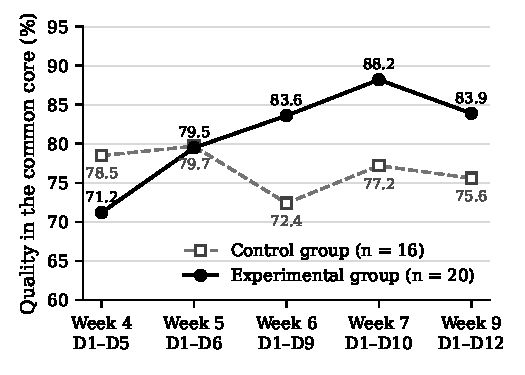
\includegraphics[width=\columnwidth]{figures/fig1_common_core.pdf}
\caption{Mean quality in the common core of dimensions at each measurement, by group. Below each week, the dimensions of the common core of that measurement (D1 to D12 following the rubric numbering). Week 8 was not measured.}
\label{fig:core}
\end{figure}

\subsection{Argumentative Quality of the Problem Description and the Justification}

In week 4, 33 complete problem descriptions and 25 complete justifications were analyzed, and in week 7, 36 of each. The model identified a median of 5 author claims per problem description; 70.4\% of the claims had at least one datum, 6.5\% a warrant, 2.2\% a backing, 5.4\% a qualifier, and 0.5\% a rebuttal, and in the justifications 66.2\% had data and 5.5\% warrants. Of the links, 57.3\% joined units from different paragraphs. Thirty-two of the 33 problem descriptions were at level 2 of Erduran \emph{et al.} \cite{erduran2004}, which corresponds to claims with grounds and no rebuttal. In week 7 the profile persisted: 81.2\% of the claims in the problem description had data and 7.6\% warrants; in the justification, 74.5\% and 4.5\%. The median elaboration index of the problem description went from 16.7\% to 20.0\% and that of the justification from 15.0\% to 18.0\%. The change in the index between the first and the last measurement with the section complete was not greater in the experimental group for the problem description, but it was for the justification (Table~\ref{tab:argument}), so H5 was partially accepted. With the structural index, which takes only seven values, $H_0$ was not rejected in either section (adjusted $p = .645$ and .189). The elaboration index was unrelated to the quality of the corresponding rubric dimension (problem description: $\rho = .04$ and .05; justification: $\rho = .02$ and .22, in weeks 4 and 7), which indicates that it captures information different from what the rubric verifies.

\begin{table*}[!t]
\caption{Argumentative Elaboration Index by Section and Group, Week 4 to Week 7}
\label{tab:argument}
\centering
\footnotesize
\begin{tabular}{L{2.6cm}L{2.8cm}cccccc}
\toprule
Section & Group & $Mdn$ W4 & $Mdn$ W7 & $Mdn$ change & $U$ & $p$ (Holm) & $\delta$ \\
\midrule
\multirow{2}{*}{Problem description} & Control ($n = 16$) & 18.4 & 20.0 & $+2.5$ & \multirow{2}{*}{156.5} & \multirow{2}{*}{.551 (.551)} & \multirow{2}{*}{$-.02$} \\
 & Experimental ($n = 20$) & 16.7 & 20.0 & $+3.1$ & & & \\
\addlinespace
\multirow{2}{*}{Justification} & Control ($n = 16$) & 15.2 & 15.3 & $-1.4$ & \multirow{2}{*}{230.0} & \multirow{2}{*}{.013 (.027)} & \multirow{2}{*}{$+.44$} \\
 & Experimental ($n = 20$) & 10.0 & 20.0 & $+3.1$ & & & \\
\bottomrule
\end{tabular}
\\[2pt]
\parbox{0.92\textwidth}{\raggedright\scriptsize Elaboration index in percent: mean, over the claims of the section, of the proportion of the five supporting components each claim has. The change is computed between the first and the last measurement at which the section is complete. One-sided Mann--Whitney $U$ test ($H_1$: the change is greater in the experimental group), with the $p$ value adjusted by Holm's method for the two sections; $\delta$ = Cliff's delta.}
\end{table*}

\subsection{Effect of the System on Methodological Quality}

Quality in the common core of each measurement changed, between week 4 (D1--D5) and week 9 (D1--D12), by $+12.6$ points on average ($SD = 11.0$) in the experimental group and by $-2.9$ points ($SD = 12.6$) in the control group. The changes of both groups were normal (Shapiro--Wilk, $p = .810$ and .795) with homogeneous variances (Levene, $p = .568$). The difference corresponds to a Cohen's $d$ of 1.32 (95\% CI $[0.60, 2.05]$; pooled standard deviation of 11.7 points), a large effect whose lower bound corresponds to a medium effect, and the one-sided Student's $t$ test yielded $t(34) = 3.94$, $p < .001$; $H_0$ of the general hypothesis was rejected. By dimension, the effect in favor of the experimental group was at least medium in eight of the twelve dimensions of the final core (Table~\ref{tab:effect}); it was negligible in the title and the consistency matrix, and favorable to the control group in the justification. On what each project had already written in week 4, the effect was negligible ($d = -0.06$; 95\% CI $[-0.72, 0.59]$).

\begin{table*}[!t]
\caption{Effect Size of the System by Rubric Dimension}
\label{tab:effect}
\centering
\footnotesize
\begin{tabular}{L{3.4cm}L{2.4cm}ccrrL{2.6cm}L{1.8cm}}
\toprule
Dimension & Measure & $n_{\mathrm{CG}}$ & $n_{\mathrm{EG}}$ & CG $M$ (\%) & EG $M$ (\%) & $d$ [95\% CI] & Magnitude \\
\midrule
D1 Title & Change W4--W9 & 16 & 20 & 3.8 & 7.0 & $0.14$ $[-0.52, 0.80]$ & Negligible \\
D2 Problem description & Change W4--W9 & 16 & 18 & $-3.1$ & 28.5 & $1.03$ $[0.31, 1.75]$ & Large \\
D3 Problem formulation & Change W4--W9 & 14 & 18 & $-5.7$ & 15.6 & $0.72$ $[0.00, 1.44]$ & Medium \\
D4 Objectives & Change W4--W9 & 15 & 18 & 0.0 & 6.3 & $0.97$ $[0.25, 1.70]$ & Large \\
D5 Justification & Change W4--W9 & 14 & 11 & 15.5 & 7.6 & $-0.32$ $[-1.12, 0.47]$ & Small \\
D6 Limitations & Level in W9 & 16 & 20 & 72.9 & 86.7 & $0.66$ $[-0.01, 1.34]$ & Medium \\
D7 Theoretical framework & Level in W9 & 15 & 20 & 81.7 & 92.5 & $0.86$ $[0.16, 1.55]$ & Large \\
D8 Hypotheses & Level in W9 & 16 & 20 & 74.0 & 85.8 & $0.40$ $[-0.26, 1.06]$ & Small \\
D9 Variables & Level in W9 & 16 & 20 & 76.4 & 92.2 & $0.92$ $[0.23, 1.61]$ & Large \\
D10 Consistency matrix & Level in W9 & 16 & 20 & 85.9 & 83.8 & $-0.10$ $[-0.76, 0.56]$ & Negligible \\
D11 Research type & Level in W9 & 10 & 16 & 44.0 & 65.0 & $0.81$ $[-0.01, 1.63]$ & Large \\
D12 Research design & Level in W9 & 8 & 16 & 32.1 & 50.9 & $0.84$ $[-0.04, 1.72]$ & Large \\
\bottomrule
\end{tabular}
\\[2pt]
\parbox{0.92\textwidth}{\raggedright\scriptsize CG = control group; EG = experimental group. For the baseline dimensions (D1--D5) the change in achievement between week 4 and week 9, in percentage points, is compared among the projects that had written them at both measurements; for dimensions incorporated later, the achievement in week 9 among the projects that wrote them. $d$ = EG $-$ CG; magnitude according to Cohen \cite{cohen1988}: negligible below 0.20, small from 0.20, medium from 0.50, large from 0.80.}
\end{table*}

\section{Discussion}

The study found that the projects of the group with access to the multi-agent system evolved significantly more favorably than those of the group with traditional advising alone, with a large effect on the change in quality in the common core of dimensions ($d = 1.32$). Two qualifications delimit that finding. First, the improvement was not exclusive to the experimental group: the quality of what had already been written increased in both groups to a similar extent, which indicates that the progress of the course, the advising, and in-class feedback act on both, and that the effect of the system concentrated in the problem description and in the quality with which the dimensions incorporated during the intervention (limitations, theoretical framework, variables, research type, and design) were written. The system is associated more with the quality with which new material is written than with the correction of material already written. Second, the effect must be interpreted against the usual practice of the course and not against the absence of tools, because the study neither restricted nor recorded the use of other artificial-intelligence tools in either group.

The result is in line with J.\ Du \emph{et al.} \cite{duj2025}, who reported a greater relative learning gain with a system of debate among agents, although for content learning rather than for the quality of a research document, and contrasts with Apol\'in Montes \emph{et al.} \cite{apolin2024}, who, with a nonequivalent control group and two measurements, found no differences in the production of academic texts with a general-purpose conversational model. The divergence is consistent with the advisors' diagnosis and with the qualitative antecedents: the functions expected from a support tool, coherence review among problem, objectives, variables, and hypotheses and evidence-based suggestions, exceed the capacity of a generic conversational agent, which tends to operate as a dispenser of resources \cite{ortega2021} or to fail with complex content questions \cite{arredondo2020}. Unlike the pre-experimental design of Hinojosa Mamani \emph{et al.} \cite{hinojosa2024}, which attributed the improvement to the intervention without a comparison group, the design with a control group and five measurements made it possible to separate the improvement common to both groups from that associated with the system and to observe that the trajectories separate from week 6 and that the advantage persisted five weeks after the baseline measurement, which responds to the recommendation of Deng \emph{et al.} \cite{deng2025} to evaluate these effects over time. In terms of measurement, the intermediate methodological level observed at baseline (between 65\% and 67\% of the applicable criteria met) coincides with the merely acceptable quality that Estrada Araoz \emph{et al.} \cite{estrada2022} found in approved theses, and the concentration of unmet criteria in the problem description confirms with direct measurement what the advisors attributed to students starting from the technological solution.

The absence of a relation between the level of use and improvement within the experimental group requires interpreting the effect as that of having the system available and not as a dose--response relationship. Use was low and concentrated in a few projects, a pattern compatible with the limited adoption documented by Arredondo Castillo \cite{arredondo2020} and with the usage records without a link to quality reported by Artiles Rodr\'iguez \emph{et al.} \cite{artiles2021}; S\'anchez-Vera \cite{sanchezvera2025} further found that moderate use of a specialized chatbot was associated with better results and that excessive use added no further improvement, which suggests that the relation between dose and outcome is not linear. Only one of the four projects with the highest use is among the five that improved most, so the number of queries does not by itself capture how each student incorporated the system's responses into the project. On the argumentative plane, the claims of both groups are supported mainly by data and rarely by warrants, backings, or rebuttals, a profile that persisted from week 4 to week 7 and that sharpens the superficial problem statement described by the advisors. The elaboration index of the justification increased more in the experimental group, but not that of the problem description, and its independence from the rubric indicates that a section can meet the required criteria without supporting its claims, information the rubric does not capture and which, following Wambsganss \emph{et al.} \cite{wambsganss2020}, could orient mentoring toward warrants and backing.

With respect to the state of the art, the study contributes the first controlled and longitudinal evidence, in a real engineering course in Peru, on a multi-agent system specialized in methodological mentoring, with an instrument validated by expert judgment, an automated evaluator with consistency reported at every measurement, and a computational assessment of the argumentation of the project sections. It does not surpass the state of the art in terms of generalization: the sample size, the assignment of intact sections, and the partial baseline homogeneity limit the external and internal validity of the between-group comparisons. Table~\ref{tab:gaps} summarizes the extent to which the results cover the identified gaps; none is declared closed, since the methodological dimensions, the most demanding ones, are not yet developed in most projects and the relation between use and improvement has not been established.

\begin{table}[!t]
\caption{Research Gaps Addressed and Degree of Coverage}
\label{tab:gaps}
\centering
\footnotesize
\begin{tabular}{cL{2.7cm}L{2.9cm}L{1.25cm}}
\toprule
SO & Gap & Contribution of the study & Coverage \\
\midrule
1 & Scarce evidence from the engineering advisor's perspective and no section-level diagnosis at the project stage & Interviews with six advisors with saturation in six categories; deficiencies by section, operational limitations, and expected functionalities & Substantial (70--80\%) \\
2 & Quality measured at a single moment, without evolution by component & Same instrument applied to the same projects at five measurements; achievement by dimension at each one & Partial (50--55\%) \\
3 & Usage logs not linked to the quality of research products & Dose of use per project and week linked to the change in quality; no positive relation & Partial (45--50\%) \\
4 & Predominance of pretest--posttest designs; little controlled evidence on specialized multi-agent systems & Five measurements compared with a mixed-effects model; large effect with a control group & Partial (50\%) \\
5 & Computational assessment of argumentation developed on essays and at a single moment & Argumentation index with cross-paragraph links and automatic verification, measured at four points and related to the rubric & Substantial to partial (50--65\%) \\
\bottomrule
\end{tabular}
\\[2pt]
\raggedright\scriptsize SO = specific objective. Coverage scale: 40\% to 50\%, partial; 65\% to 80\%, substantial with pending components; 85\% to 100\%, closed. Overall coverage of the ten gaps: 56.5\%.
\end{table}

\subsection{Limitations}

The design worked with intact sections without random assignment of projects, and baseline homogeneity was partial: the control group started with higher traceability and a moderately higher core quality ($g = -0.65$), so part of the convergence may be due to regression to the mean; for this reason the comparisons relied on the change of each project relative to its own baseline and on a model that estimates level and slope separately. Section-specific factors, such as composition, class day and pace, external advising, or the use of other artificial-intelligence tools, were not controlled; in week 6, moreover, advising to both groups was minimal. The results correspond to a single faculty and to five measurements of a series that continues until the first complete version of the projects, and the methodological dimensions are not yet developed enough to analyze their evolution. The evaluation system was the only administrator of the rubric: its validity rests on the content validation of the instrument and on the dichotomous nature of the items, but its scores were not contrasted with human raters. The three judges belong to the same model family and at least one of them is among the models used by the mentoring system, so the panel does not neutralize self-preference bias \cite{panickssery2024}; the risk was mitigated with temperature 0, a fixed seed, dichotomous criteria, and majority voting, without eliminating it. Inter-judge variability was moderate (Fleiss' kappa between .46 and .66). The argumentation index records the presence of components and not their soundness, its test--retest stability was moderate (ICC = .77), and its contrast with human annotation is pending; the partial acceptance of H5 depends on the continuous index and should be interpreted with caution.

\subsection{Future Work}

We suggest replicating the design in other schools and universities with larger samples and cluster randomization; completing the longitudinal series up to the final version of the projects to analyze the methodological dimensions; contrasting the panel's scores with human raters on a subsample, with bootstrap confidence intervals; composing judge panels with models from different families and distinct from the generating model; recording the use of other artificial-intelligence tools in both groups; analyzing the same data with usage indicators that capture the effective incorporation of the system's responses into the document; and validating the argumentation index with human annotation of the same sections.

\section{Conclusion}

\begin{enumerate}
\item The qualitative diagnosis identified the problem formulation and the methodological framework as the sections with the highest incidence of errors, and the punctual nature of advising as the main structural limitation of traditional mentoring; the functionalities advisors expect from a support tool exceed the capacity of a generic conversational agent and support the choice of a specialized multi-agent architecture anchored in a rubric.
\item The methodological quality of the projects increased significantly between week 4 and week 9 in 32 of 36 projects (median $+13.0$ points; $p < .001$), in both groups, with baseline deficiencies concentrated in the problem description; measurement rested on a rubric with content validity (Aiken's $V$ between .81 and 1.00).
\item The level of use of the system, low and concentrated in a few projects (215 queries), was unrelated to the improvement in quality in the experimental group ($\rho = -.14$; $p = .725$), so the effect shows no dose--response relationship.
\item Quality in the dimensions developed by both groups evolved significantly more favorably in the experimental group, with a weekly slope 3.10 points higher ($p < .001$); the difference originated in the dimensions incorporated after the baseline measurement.
\item The claims of the problem description and the justification are supported by data and rarely by warrants, backings, or rebuttals; the elaboration index of the justification increased more in the experimental group (adjusted $p = .027$), but not that of the problem description, so H5 was partially accepted.
\item The multi-agent system had a positive, statistically significant, and large effect on the methodological quality of the thesis projects ($d = 1.32$; 95\% CI $[0.60, 2.05]$; $p < .001$), concentrated in the problem description and in the dimensions written during the intervention, interpreted as the effect of having the system available relative to the usual practice of the course. As a practical implication, automated mentoring systems should prioritize strengthening the description and formulation of the problem, and the faculty should consider mechanisms to standardize criteria between advisors and examining boards, whose divergence reached full saturation in the diagnosis.
\end{enumerate}

\section*{Acknowledgment}

The authors thank the instructors and advisors of the Faculty of Engineering at UPAO who took part in the interviews and in the validation of the instrument, the instructor of the Research Project course for facilitating the study in his sections, and the students who authorized the evaluation of their projects. The language models described in Section~II are part of the object of study; no generative artificial intelligence was used to make research decisions.

\section*{Data and Code Availability}

The source code of the mentoring system is available at \url{https://github.com/Mclever2/MentorIA-Tesis}. The 100-item rubric with its Aiken's $V$ coefficients, the interview guide, the per-project results at each measurement, the panel consistency statistics, and the usage logs aggregated by project and week are provided as supplementary material.

\bibliographystyle{IEEEtran}
\bibliography{references}

\begin{IEEEbiographynophoto}{Clever Josu\'e Aguilar Idrogo}
is a candidate for the professional degree of Computer and Systems Engineer at Universidad Privada Antenor Orrego, Trujillo, Peru. His research interests include multi-agent systems based on large language models, retrieval-augmented generation, and artificial intelligence applied to higher education.
\end{IEEEbiographynophoto}

\begin{IEEEbiographynophoto}{Alessia Vidamilagros Aguilar Alayo}
is a candidate for the professional degree of Computer and Systems Engineer at Universidad Privada Antenor Orrego, Trujillo, Peru. Her research interests include educational technology, automated assessment of academic writing, and intelligent systems.
\end{IEEEbiographynophoto}

\begin{IEEEbiographynophoto}{Walter Manuel Cueva Ch\'avez}
is a professor with the Faculty of Engineering, Universidad Privada Antenor Orrego, Trujillo, Peru, where he advises undergraduate thesis projects in the Computer and Systems Engineering program. His research interests include research methodology, intelligent systems, and software engineering.
\end{IEEEbiographynophoto}

\end{document}
